\begin{chapterquote}
  ``Anything one man can imagine, other men can make real.''
  \quoteauthor{Jules Verne}
%  ``All writers are vain, selfish and lazy, and at the very bottom of their
%   motives lies a mystery. Writing a book is a long, exhausting struggle,
%   like a long bout of some painful illness. One would never undertake such
%   a thing if one were not driven by some demon whom one can neither resist
%   nor understand.''
%  \quoteauthor{George Orwell}

% ``I recognize that many physicists are smarter than I am -- most of them
% theoretical physicists. A lot of smart people have gone into theoretical physics,
% therefore the field is extremely competitive. I console myself with the thought
% that although they may be smarter and may be deeper thinkers than I am, I have
% broader interests than they have.''
% \quoteauthor{Linus Pauling (1901-1994)}
\end{chapterquote}



\chapter{Introduction}


\section{The need for hypersonic airbreathing propulsion}

Manned and unmanned space traveling has to date been achieved using rocket propelled
multi-staged systems. This approach to space transportation has proven to be viable
but rather inefficient: more than 60 percent of the take-off mass of the space vehicle
is the oxidant supply \cite{book:1994:pratt}, compared to only 5 percent of the take-off
mass being the payload. It follows that the replacement of the rocket engine with an
airbreathing engine for the early stages of flight would drastically reduce the
amount of oxidant needed to be carried on board. Space transportation costs would
then be significantly reduced due to the much increased percentage of the take-off
mass that could be allocated to the payload.

In order to be an efficient substitute to the rocket engine, the airbreathing engine
must be able to operate throughout the flight Mach number envelope 0-15. Although a
ramjet could be used up to Mach numbers of 6, the cycle performance of this type of
engine deteriorates at hypersonic velocities, due to the high losses in stagnation
pressure encountered through the flow deceleration process prior to the subsonic
combustion region. Further, decelerating the flow to subsonic conditions
through gasdynamics means alone, even when ensuring that the process is isentropic,
would induce a considerably high combustor entrance temperature
at high flight Mach number (see Figure \ref{fig:combustor_entrance}).
A high temperature at the combustor entrance would dissociate the incoming air, prevent
the combustion process to release the maximum heat from the fuel/air mixture,
and impose excessive heat
loads on the flight vehicle. Consequently, hypersonic airbreathing propulsion research has
focused in recent years on supersonic combustion, with particular emphasis
given to supersonic diffusive burning engines \cite{aiaaconf:2001:mcclinton}
(also referred to as
\emph{s}upersonic \emph{c}ombustion \emph{ramjets}, or scramjets). While showing great
promise, the scramjet design is hampered by slow diffusive burning in the combustor,
resulting in a longer combustion chamber required to mix adequately the fuel with the
incoming air, and release the available energy of the mixture. This translates into a
more massive structure of the engine and a more complicated cooling system, which
decreases the performance of this type of flight vehicle.
%
\begin{figure}[!h]
   \center
   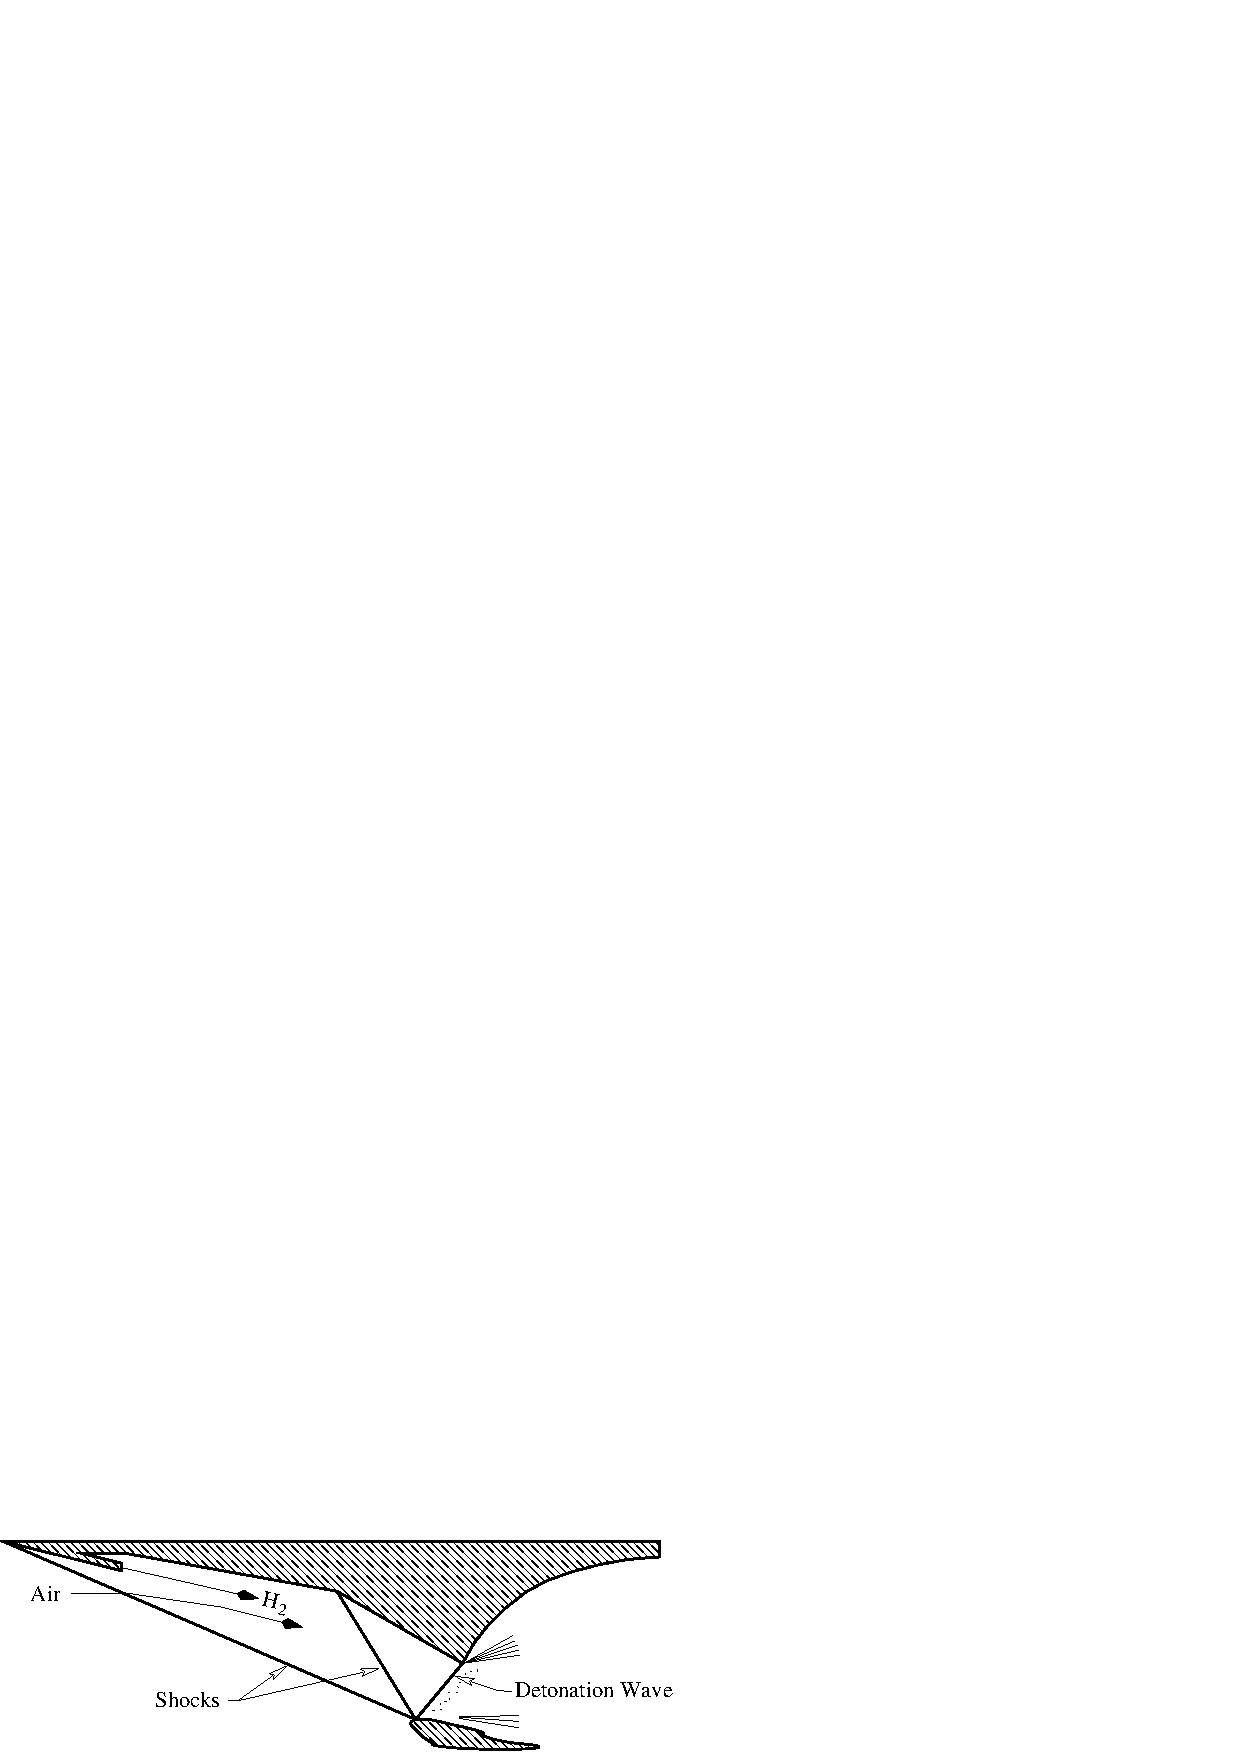
\includegraphics[width=4.0\lengthfigure]{fig1/shcramjet.pdf}
   \caption{External compression shcramjet schematic.}
   \label{fig:shcramjet}
\end{figure}
%



\section{The \emph{sh}ock-induced \emph{c}ombustion \emph{ramjet} (shcramjet)}


First proposed by Roy \cite{misc:1946:roy}, an alternate hypersonic propulsion concept
that aims at increasing the fuel
efficiency and thrust of the scramjet is the oblique detonation wave ramjet, also
referred to as the \emph{sh}ock-induced \emph{c}ombustion \emph{ramjet} (shcramjet)
\cite{aiaabook:2001:sislian,nasa:2000:jones}, as shown
in Figure \ref{fig:shcramjet}.  The massive
combustion chamber is avoided by burning the fuel/air mixture through a thin detonation
wave, with the fuel injected  in the inlet near the leading edge of the vehicle. This
reduces the weight of the engine and takes full advantage of the typically long inlets
found at hypervelocities.

Preliminary predictions of the performance of the shcramjet were
performed through
simplified one-dimensional analyses (see Sargeant and Gross \cite{misc:1959:sargeant}
or Dunlap \etal\ \cite{misc:1978:dunlap}). More detailed analytical
models ensued by Townend \cite{misc:1970:townend},
Morrison \cite{nasa:1978:morrison,nasa:1980:morrison},
and Ostrander \etal\ \cite{aiaaconf:1987:ostrander} to
assess the on-design and even off-design performance of the flight vehicle.
Later followed inviscid simulations of planar and axisymmetric
shcramjets by Sislian \etal\ using numerical methods based on exact and approximate
Riemann solvers
\cite{aiaaconf:1989:sislian,aiaaconf:1992:atamanchuk} also including
the non-equilibrium chemical kinetics equations for hydrogen/air combustion
\cite{jpp:1998:dudebout}.
The results obtained through the numerical studies confirm the encouraging
performance of the shcramjet found in previous analytical
work: (i) the shcramjet is seen to perform better than
a scramjet at high flight Mach number, and (ii) the shcramjet delivers a
fuel specific impulse superior to that of a rocket
up to a flight Mach number of 22 (see Ref.~\cite{jpp:1998:dudebout}).


Besides neglecting viscous effects, all of the above-mentioned studies assume
that no premature ignition occurs prior to the detonation wave, and
that the fuel and air are mixed in stoichiometric proportions prior to the
detonation wave.
To the author's knowledge, the only published work outlining the effect of
incomplete fuel/air mixing on the shcramjet performance is
Ref.~\cite{jpp:2000:sislian}, where Sislian \etal\ 
assess the impact of incomplete mixing on the net thrust by fixing
a non-uniform equivalence ratio distribution at the inlet entrance. It is observed that
an equivalence ratio distribution varying from $\phi \approx 2.4$ near the wall
to $\phi\approx 0.02$ in the freestream decreases the fuel specific impulse
by as much as $40\%$ in the flight Mach number range $9 \leq {\rm M}_{\rm flight} \leq 24$.
Due to the high sensitivity of the thrust of the shcramjet to incomplete fuel/air mixing,
achieving adequate fuel/air mixing in the inlet while preventing premature
ignition is one of the main technical challenges that needs to be
resolved to establish the shcramjet as a viable hypersonic airbreathing
flight vehicle.


%
\begin{SCfigure}
   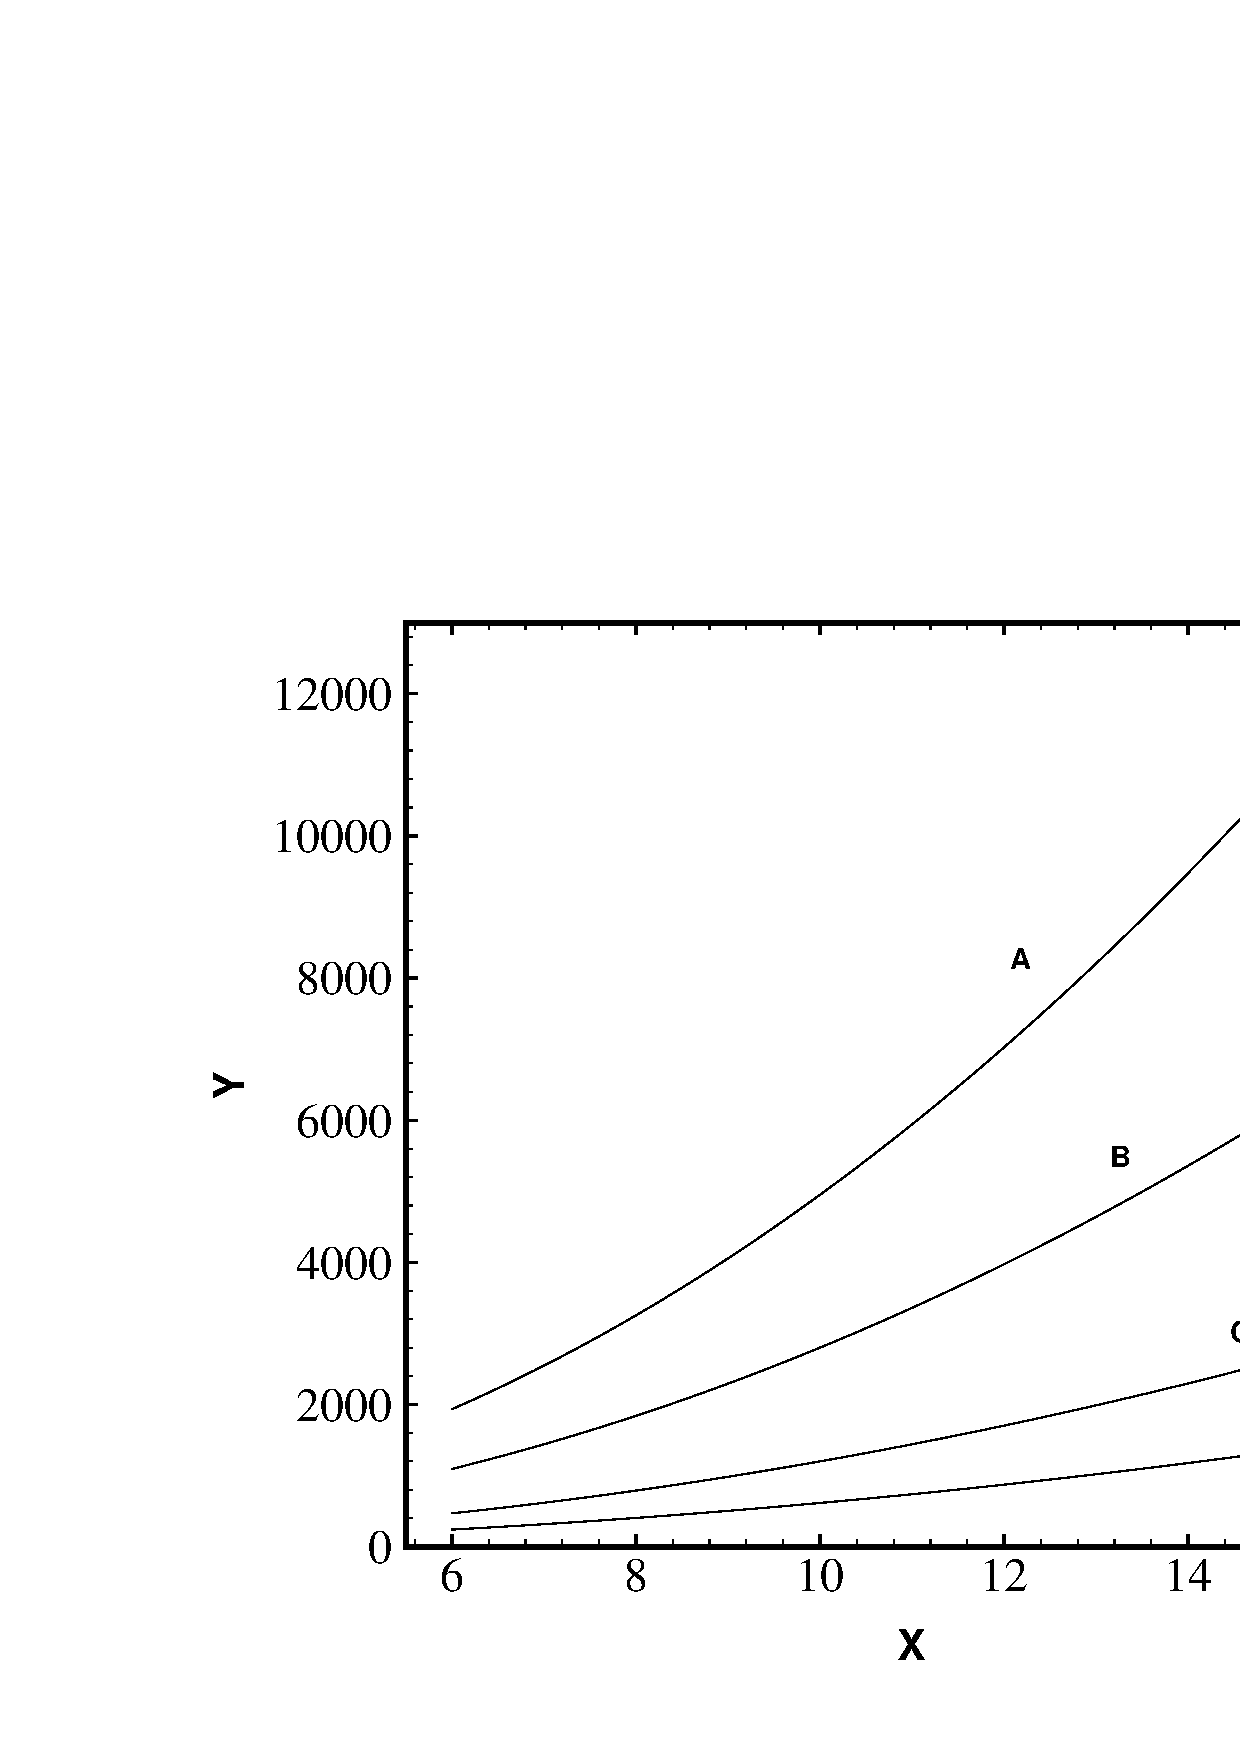
\includegraphics[width=3.8\lengthfigure]{fig1/combustor_entrance.pdf}
   \caption{Temperature at the combustor entrance versus the flight Mach
            number, assuming the ambient air temperature is 240~K, $\gamma=1.4$,
            and the deceleration process is isentropic.}
   \label{fig:combustor_entrance}
\end{SCfigure}
%


\section{Fuel/air mixing at hypervelocities}



Besides preventing premature ignition, it is desirable for
fuel injection in a hypersonic vehicle to be such that
most of the thrust due to the momentum
of the fuel is recovered by injecting the fuel in the same
direction as the surrounding freestream
(see Refs.~\cite{aiaa:1966:rubins,misc:1970:townend,
nasa:1978:morrison,nasa:1980:morrison}).
The need to inject fuel parallel to the surrounding freestream
direction is balanced by the need of adequate
fuel penetration in the incoming air while avoiding hard-to-cool intrusive parts.
This prompted the development of near-parallel
mixing configurations aimed at enhanced fuel penetration
and fuel/air contact surface stretching (see a recent review in
Ref.~\cite{misc:1995:gutmark} and other mixing strategies in
Refs.~\cite{jpp:1995:bushnell} and \cite{jpp:1994:bogdanoff}).


\subsection{Fuel pre-injection in scramjet inlets}


There has been a recent interest in pre-mixing the fuel with the air
upstream of the combustor to improve the mixing and burning performance  of
scramjets. Vasilev \etal\ \cite{aiaa:1994:vasilev} numerically investigate
on the fuel/air mixing in a Mach 8 inlet by means of an injector structurally detached
from the engine and placed well upstream of the inlet.
At the inlet exit,
a mixing completeness of as much as 0.6 to 0.7 is achieved without significant
stagnation pressure losses.
As a means to improve the efficiency of the heat release in scramjet combustors,
Segal \etal\ \cite{aiaa:2000:livingston,jpp:2001:owens} consider liquid
fuel pre-injection in the inlet, upstream of the combustor. They
experimentally investigate on the normal injection of
liquid fuel JP-10 behind thin pylons in a  Mach 1.6 and Mach 3.5
incoming air flow. The experimental results are representative of fuel injection
in the inlet
of a  scramjet operating in the lower end of the hypersonic flight regime,
where the high enthalpy incoming air flow interacts with the lower-speed fuel,
hence helping the process of liquid droplet breakup.
The use of pylons to inject gaseous hydrocarbon in a Mach 6--8
scramjet inlet is further investigated numerically by Guoskov \etal\
\cite{jpp:2001:guoskov}
who report a fuel-based mixing efficiency of 0.95 to 0.98 for
a global equivalence ratio varying between 0.3 and 0.7 respectively.
Both the experimental results by Segal \etal\ and the numerical results
by Guoskov \etal\ show that the pylons contribute
significantly to lift the liquid from the
injection surface, thus avoiding fuel in the boundary layer and potential
flashback.

%
\begin{figure}[!b]
   \center
   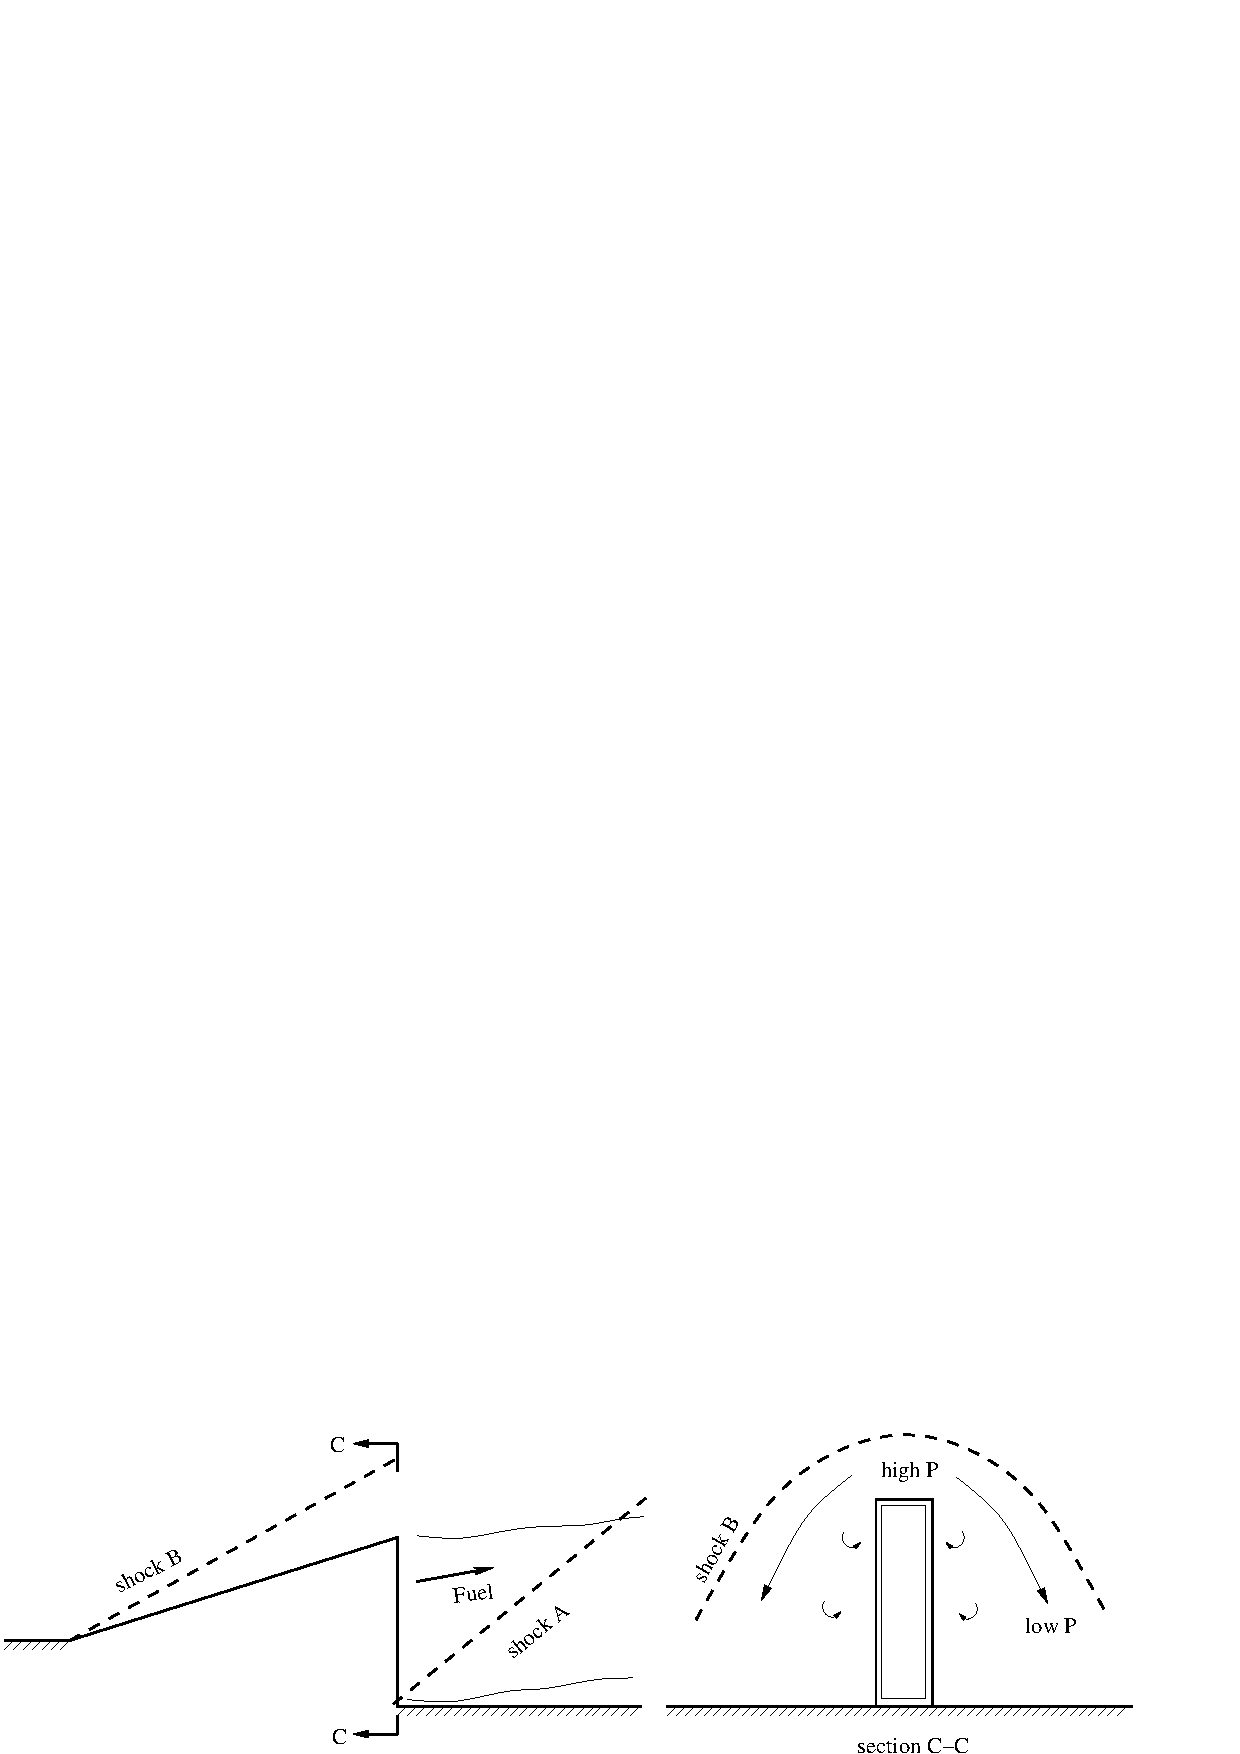
\includegraphics[width=4.6\lengthfigure]{fig1/ramp.pdf}
   \caption{Wall-mounted ramp injector schematic.}
   \label{fig:ramp-schema}
\end{figure}
%




\subsection{Choice of turbulence model}

Simple algebraic turbulence models (Cebeci-Smith and Baldwin-Lomax) were used
in almost all previous turbulent hypervelocity fuel/air mixing studies, with the
exception of a few \cite{aiaa:1998:lee,aiaaconf:1995:scherrer,jpp:1997:baurle}  where
``universal'' two-equation $k\epsilon$, $k\omega$ or $q\omega$ turbulence models were
considered. Also, the numerical investigations of inlet mixing reported so far
\cite{aiaa:1994:vasilev,jpp:2001:guoskov}
are limited to one-equation turbulence models without additional corrections
for compressibility effects.
In the present work, the Favre-averaged Navier-Stokes equations (FANS) are
closed by the low-Reynolds number $k\omega$ two-equation
turbulence model of Wilcox \cite{aiaa:1988:wilcox}. Despite its notable sensitivity
to the freestream conditions, the $k\omega$ model is preferred
to the $k\epsilon$ model due to its capability at solving
accurately the laminar sublayer of the turbulent boundary layer without the addition
of low-Reynolds number source terms \cite{aiaa:1988:wilcox}.
Aside from their inelegance, low-Reynolds
number source terms increase the stiffness of the governing equations and
require more grid points to be resolved properly. Further, the $k\epsilon$ model does
not predict correctly the growth of the boundary layer under an adverse pressure
gradient \cite{book:1994:wilcox}, a situation likely to occur in the inlet.
Wall functions are not used in the present study
as their accuracy is questionable in regions of
separated flow, which are present in the vicinity of the cantilevered ramp injector
and possibly in the vicinity of shock~/~boundary-layer interactions occurring
in the inlet. It is noted that improvements to the low-Reynolds number
Wilcox $k\omega$ model have been proposed recently by Menter \cite{nasa:1992:menter}
and later by Wilcox \cite{book:1998:wilcox}, in order to reduce the sensitivity of the $k\omega$
model to the freestream value of $\omega$. While showing great promise, the improved $k\omega$
models have not yet been validated as thoroughly in the literature as the low-Reynolds
number Wilcox $k\omega$ model, and are hence not considered for this study.

Among the various existing
compressibility corrections \cite{nasa:1978:sislian,thesis:1996:krishnamurty,
nasa:1994:coakley}, only the ``dilatational dissipation'' correction
\cite{misc:1990:zeman,jfm:1991:sarkar,aiaa:1992:wilcox} is retained in the
present investigation, due to a lack of experimental data justifying the presence of
other corrections. The use of the dilatational dissipation is particularly important
to predict the shcramjet inlet flowfield accurately due to the generally
high convective Mach number
in use. At a high convective Mach number,
compressibility effects are observed through experiments to restrict the growth
of the shear layer considerably \cite{jfm:1988:papamoschou,aiaabook:1991:dimotakis}.
This trend is not predicted correctly by the baseline $k\omega$ model and
a dilatational dissipation correction term needs to be introduced in the turbulence
kinetic energy equation to account for this compressibility effect. The dilatational
dissipation corrections proposed by Zeman \cite{misc:1990:zeman}
and by Sarkar \etal\ \cite{jfm:1991:sarkar} are applicable only to high
Reynolds number regions, and not in the laminar sublayer of the turbulent
boundary layer, for instance. Hence, the Sarkar and Zeman corrections are not
used for the mixing problems presented here as they result in an underprediction of
the wall shear
stress at the high flow Mach numbers typical of the shcramjet inlet. Instead,
the dilatational dissipation correction
of Wilcox \cite{aiaa:1992:wilcox} is preferred as it is shown not to alter the
shear stress over a flat plate up to a freestream Mach number of 6,
when used in conjunction with the $k\omega$ model.


\subsection{Discretization of the convection derivative}

Contrarily to the discretization of the diffusion terms which can
be accomplished through centered finite-difference stencils, the
discretization of the convection terms is problematic
(see Ch.~5 in Ref.~\cite{book:1980:patankar}).
A successful approach at discretizing the convection derivative is
through upwinding, as first proposed by Courant \etal\ \cite{misc:1952:courant}
for the solution of a scalar advection equation.
For the gas dynamics equations, the upwinded method is generalized by
Godunov \cite{misc:1959:godunov}, through the exact solution of a fictitious
Riemann problem midway between nodes. A simpler, linearized approximate Riemann
solver based on eigenvalue splitting is later proposed by
Roe \cite{jcp:1981:roe}. The Roe scheme has
the property of reverting to a first-order upwind stencil in case of locally
supersonic flow, and of reverting to a centered finite difference scheme with
matrix dissipation when the local velocity is much smaller than sonic.
Probably due to its relative
ease of extension to different governing equations, and its ease of linearization
when used in conjunction with an implicit scheme, the Roe scheme has
become one of the preferred Riemann-solver-type method
for compressible flow. Yee \etal\ \cite{jcp:1990:yee} extend the Roe method to
second-order accuracy
while retaining the original monoticity of the first-order method by the use
of flux limiters, resulting in increased accuracy for many flowfields. The
latter is the discretization method chosen for this study, and is
referred to hereafter as the Yee-Roe scheme. The Yee-Roe
scheme is here applied in coupled form to all transport equations, including the turbulence
kinetic energy, the specific dissipation rate of the turbulence kinetic energy,
the continuity, the momentum, and the energy
transport equations. The eigenstructure of the Roe flux Jacobian for the FANS
equations is presented.


\subsection{Pseudotime stepping}

An implicit strategy is here chosen to advance the solution in pseudotime
to steady-state, in order to relieve the constraints on the pseudotime step size
imposed by the viscous terms in flow regions where the grid spacing is small
(such as in the laminar sublayer of the turbulent boundary layer for instance).
To minimize storage requirements and the inversion effort,
a block-implicit approximate-factorization (AF) algorithm
\cite{jcp:1977:briley, aiaa:1978:beam} is used.
The convection terms are linearized assuming a frozen Roe Jacobian, while
the viscous terms are linearized following a strategy outlined
in Chang and Merkle \cite{jcp:1989:chang}.
While relatively dated (the scalar approximate-factorization
algorithm dates back almost 50 years and the block-implicit version was
first proposed in the late 1970's), block-implicit AF
is still at the heart
of many numerical methods solving the Euler or Navier-Stokes equations in the
hypersonic range (see Refs.~\cite{aiaaconf:1997:maccormack,cf:2001:maccormack}
for instance). Despite having the potential to significantly accelerate the
convergence of the baseline block implicit AF method,
Newton-Krylov and multigrid methods are rare in
present day codes aimed at solving hypersonic viscous flows. Additional difficulties
in the hypersonic range originate from strongly non-linear phenomena (such as
shock waves and chemical reactions) that hamper the performance of multigrid,
although recent advancements shed some hope that this can be remedied,
at least for certain flowfields \cite{jcp:2001:gerlinger}.


\subsubsection{Convergence acceleration through space-marching}

There is little doubt that the most efficient way to solve
supersonic or hypersonic flow with no streamwise ellipticity is
through a space-marching method, as numerous extremely efficient
marching methods developed over the years can attest (see for example Refs.
\cite{aiaaconf:1978:vigneron,aiaaconf:1986:lawrence,aiaaconf:1988:tannehill,
cf:1997:dambrosio,cf:1998:miller}). The Navier-Stokes equations at supersonic
speeds do, however, exhibit some ellipticity in the marching direction through
the streamwise viscous terms and the subsonic layer of the boundary layer,
and it is necessary for a space-marching method to ignore these mechanisms by
solving a reduced set of the original equations of motion, such as
the parabolized Navier-Stokes equations (PNS). The PNS are defined here as
the equation set obtained
from the Navier-Stokes equations by neglecting all viscous terms in the
streamwise direction and by modifying the streamwise momentum equation to
prevent any pressure
disturbance from traveling upstream, using characteristics splitting or pressure
splitting as suggested by Vigneron \etal\ \cite{aiaaconf:1978:vigneron}.
The applicability of the space-marching methods is
limited to flows with negligible streamwise ellipticity, hence preventing their
deployment to many practical flowfields.


\subsubsection{Difficulties originating from large streamwise-separated regions}

The need to tackle streamwise ellipticity prompted the development
of the ``global iteration'' space-marching methods in which
a sweep is performed several times on the entire computational
domain to permit the upstream propagation of information
(see Ref.~\cite{aiaa:2000:miller} for a detailed review).
These schemes are characterized, compared to the pseudotime marching schemes,
by a smaller memory requirement due to the storage
of temporary variables in one marching plane only and by
enhanced wave propagation mechanism in the streamwise
direction. The reduced Navier-Stokes (RNS) equations, which are derived from
the Navier-Stokes equations by ignoring all streamwise diffusion terms but
not altering the momentum convection terms,
are usually solved in this manner leading to fast convergence of subsonic/supersonic
streamwise unseparated flows \cite{aiaa:1988:power,jcp:1989:chang,aiaa:2000:yamaleev}
and even of viscous/inviscid interactions creating streamwise separation
\cite{cf:1983:rubin,aiaa:1986:barnett}. In a similar vein,
Bardina \cite{aiaaconf:1994:bardina} shows that significant reduction in work
is achievable by the use of  global marching sweeps to solve the full
Navier-Stokes equations for high-speed flows. However, if not limited to some
predetermined zones of the computational domain, the global iteration
approach loses some performance when solving large reverse flow regions,
as the number of sweeps can become excessive due to its dependence
on the size in streamwise grid lines of the separation bubble.
Further, some computing might be inefficiently
allocated to the nodes downstream of the separation bubble, \emph{prior} to its
convergence. These deficiencies can be remedied by using a space-marching
scheme solving the PNS equations until an elliptic/reverse flow region is
encountered, then switching to a global iteration RNS method (or FANS)
for the length of the
elliptic region, iterating until convergence is reached, and pursuing with
the marching PNS scheme (see Miller \etal\ \cite{aiaa:2000:miller} for instance).
However, such a strategy forces the solution of the PNS equations in certain
regions of the flowfield for which the PNS assumption might induce
appreciable errors. The accuracy of the final solution is hence strongly
dependent on the ability of the method at predicting correctly which
regions of the flowfield can be accurately predicted with the PNS equations,
and which regions require the use of the RNS (or FANS) equations.


\subsubsection{The domain rollover method}

In Ref.\ \cite{thesis:1997:underwood}, Underwood presents
a technique based on domain decomposition which is
aimed at improving the generality of the above-outlined PNS
methods with embedded elliptic solvers. The technique
is dubbed ``domain rollover'' and can be summarized as follows.
Prior to the iterative process, the physical domain is divided into a
series of subdomains in the streamwise
direction. Then, the FANS equations are iterated in
pseudotime on a solution domain which is
composed of a certain number of adjacent subdomains (the number of subdomains
being user-specified). When the residual
in the upstream subdomain part of the solution domain falls below a user-specified
convergence threshold, the solution domain advances by one subdomain in the
streamwise direction. To correctly capture regions of streamwise ellipticity,
it must hence be ensured before starting the iterative process that each
subdomain is large enough to contain the streamwise-elliptic regions
that are expected to form in its interior. This is necessary due to the lack
of ``streamwise ellipticity sensors'' at the upstream and downstream
boundaries of the solution domain. The lack of sensors prevents a locally elliptic
region to outgrow the solution domain boundaries. Therefore,
similarly to the PNS methods with embedded elliptic solvers,
the success of the domain rollover method at predicting accurately flowfields
including streamwise-elliptic regions depends on the ability of the user
at predicting \apriori\ the location and size of the zones of streamwise ellipticity.








\subsubsection{The active domain method}

Recently, a novel approach at solving inviscid supersonic flow with embedded
subsonic regions has been proposed \cite{aiaa:1997:nakahashi}. The method,
named ``active domain'', consists of performing pseudotime iterations
on a small band-like computational domain that advances in the streamwise direction
every time the residual of the active domain near the upstream
boundary falls below a user-defined threshold.
Using sensors based on the streamwise component of the Mach number,
the active domain boundaries automatically surround any
locally subsonic region, on which sufficient iterations are performed to reach
steady-state. When the residual inside the subsonic region decreases below
the user-defined threshold, the active domain advances past the subsonic region
further downstream. By marching in the streamwise direction, the active domain
results in a decrease
in work of up to 10 times compared to standard pseudotime marching methods
for several inviscid problems. However, the ability of the active domain at solving accurately a
streamwise elliptic region is limited by the accuracy of the sensor responsible for the
upstream movement of the upstream boundary of the active domain. Extension
of the active domain method to viscous flow is hampered by the
difficulty of formulating a streamwise ellipticity sensor that captures
all significant upstream propagating waves while restricting the size of
the active domain to a minimum. Success has been reported in solving
viscous flow without streamwise separation by maintaining the active domain
width equal to the height of the boundary layer \cite{aiaaconf:1999:morino}.
However, to the author's knowledge, the active domain method has not yet been extended
to streamwise separated flows.



\subsubsection{A new convergence acceleration technique}

This thesis proposes an alternate form of the active domain method,
named the ``marching window'' algorithm, that can be used to solve the FANS
equations for problems including streamwise separated flows. Similarly to the
active domain, the marching window
performs localized pseudotime stepping on a subdomain
composed of a sequence of streamwise planes. The width of the marching window
decreases to only a few planes in regions of quasihyperbolic flow
and increases to the size of the streamwise-elliptic region when encountered.
However, in sharp contrast to the active domain algorithm (and also to the domain
rollover algorithm), the marching window is
strictly a convergence acceleration technique as it guarantees the residual of
all nodes to be below the user-defined threshold when convergence is attained.
This is accomplished by keeping the residual upstream of the marching
window subdomain updated at all times, and by positioning the upstream boundary
such that the residual of all nodes upstream is below the user-defined threshold.
This results in an algorithm that captures all upstream
propagating waves affecting the residual significantly. The upstream
propagating waves can originate from (but are not necessarily limited to) large subsonic
pockets, streamwise separation, streamwise viscous fluxes, or the flux limiters in
the streamwise convection flux derivative, for instance. Further,
to enhance the performance of the algorithm,
a sensor based on the Vigneron splitting \cite{aiaaconf:1978:vigneron}
is developed to advance the downstream boundary
when significant streamwise ellipticity is detected.


To assess the performance of the marching window, several numerical experiments are
presented in Chapter~\ref{chapter:numerical_method}
ranging from the inviscid solution
of a supersonic inlet with a blunt leading edge to turbulent shock boundary layer interactions
with considerable streamwise flow separation solved with the FANS
equations closed by the $k\omega$ turbulence
model of Wilcox \cite{aiaa:1988:wilcox}. A time accurate turbulent flow field using
dual time stepping is also investigated. In all cases, a comparison between the
marching window cycle, the active domain cycle (for the inviscid case only),
and the standard pseudotime marching cycle
is made on the basis of CPU time, effective iterations, and storage.


